\section{Lower bounds}



\begin{proposition}
	The "target reachability problem" (asking whether there is a run in which all agents reach a state $q_f$) is undecidable for BNRA with two registers.
\end{proposition}

\ifproofs
\begin{proof}
	We present a reduction of the "halting problem" for "Minsky machines" to "target reachability problem" for BNRA.
	
	A "Minsky Machine" is a tuple $M= (\Loc, \Delta, \Cpt, \ell_0, \ell_f)$ where $\Loc$ is a finite set of locations, $\Cpt = \{\cpt_1, \cpt_2\}$ is a set of two counters, $\Delta \subseteq \Loc \times (\{\dec{\cpt}\}_{\cpt \in \Cpt} \cup \{\inc{\cpt}\}_{\cpt \in \Cpt} \cup \{\testz{\cpt}\}_{\cpt \in \Cpt} ) \times \Loc$ is a finite set of transitions, $\ell_0 \in \Loc$ is an initial location, and $\ell_f \in \Loc$ is a final location. A \emph{configuration} of a Minsky machine is a tuple $(\ell, v_1, v_2) \in \Loc \times \nats \times \nats$ where $v_1$ (resp. $v_2$) stands for the value of the counter $\cpt_1$ (resp. $\cpt_2$). The initial configuration is the configuration $(\ell_0, 0, 0)$.
	For two configurations $(\ell, v_1, v_2)$ and  $(\ell', v'_1, v'_2)$, we note $(\ell, v_1, v_2) \stepMM{} (\ell', v'_1, v'_2)$ if $\exists \delta \in \Delta$ such that one of the following condition holds:
	\begin{itemize}
		\item $\delta = (\ell, \inc{\cpt_i}, \ell')$ and $v'_i = v_i+1$, $v_{3-i} = v'_{3-i}$;
		\item $\delta = (\ell, \dec{\cpt_i}, \ell')$ and $v'_i = v_i-1$, $v_{3-i} = v'_{3-i}$;
		\item $\delta = (\ell, \testz{\cpt_i}, \ell')$ and $v'_i = v_i = 0$, $v_{3-i} = v'_{3-i}$.
	\end{itemize}
%	We will note $\stepMM{}$ for $\bigcup_{\delta \in \Delta} \stepMM{\delta}$. 
	An execution of the machine is a sequence $(\ell_1, v_1^1, v_2^1) \stepMM{} (\ell_2, v_1^2, v_2^2) \stepMM{} \dots \stepMM{} (\ell_k, v_1^k, v_2^k)$. We say that an execution is initial if it starts with the initial configuration.
	The "halting problem" asks whether there exists an initial execution ending with a configuration $(\ell_f, v_1, v_2)$ where $v_1$, $v_2$ are any values in $\nats$. This problem is well-known to be undecidable.
	%\luin{to make the proof easier, one might require that there is no two transitions doing the same operation from a same location, this does not change the undecidability}
	
	
%	\begin{figure}
%		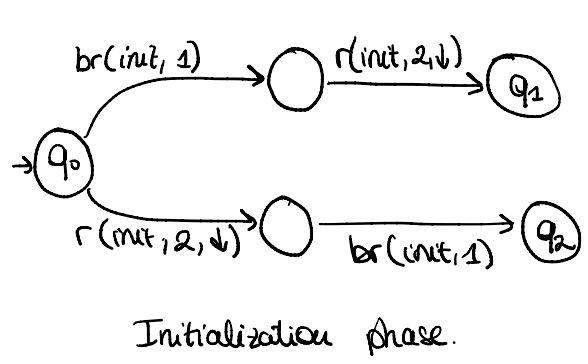
\includegraphics[scale = 0.25]{Figures/init.png}
%		\caption{init}\label{fig:target:init}
%	\end{figure}

\begin{figure}
	\begin{tikzpicture}[xscale=0.5,AUT style,node distance=2.1cm,auto,>= triangle
	45]
	\tikzstyle{initial}= [initial by arrow,initial text=,initial
	distance=.7cm]
	%	\tikzstyle{accepting}= [accepting by arrow,accepting text=,accepting
	%	distance=.7cm,accepting where =right]
	
	\node[state,initial, minimum width=0.1pt] (0) at (0,0) {$q_0$};
	\node[state] [right of=0, yshift=20] (x) {1};
	\node[state] [right of=0, yshift=-20] (y) {2};
	\node[state] [right of=x, xshift=10] (1) {$q_1$};
	\node[state] [right of=y, xshift=10] (2) {$q_2$};
	
	\path[->, bend left=10] 	
	(0) edge node[above, xshift=-10] {$\br{init}{1}$} (x)
	;
	\path[->, bend right=10] 	
	(0) edge node[below, xshift=-10] {$\rec{init}{2}{\enregact}$} (y)
	;
	\path[->] 	
	(x) edge node {$\rec{init}{2}{\enregact}$} (1)
	(y) edge node {$\br{init}{1}$} (2)
	;
\end{tikzpicture}
	\caption{init}\label{fig:target-init}
\end{figure}

%	\begin{figure}
%		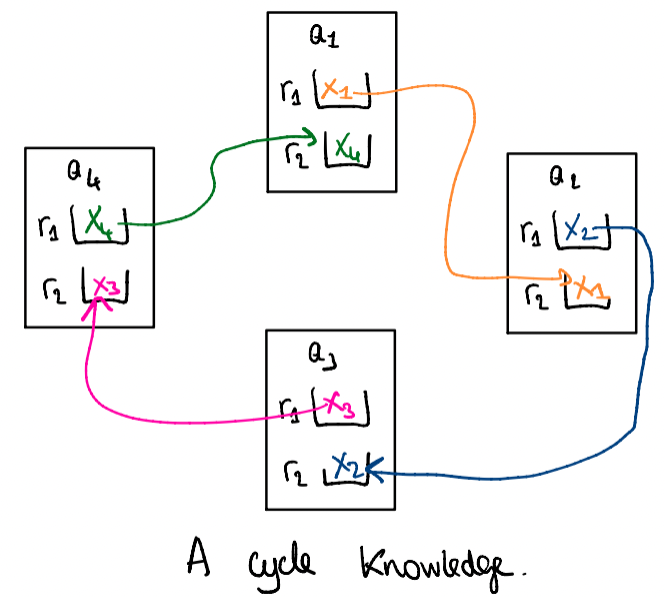
\includegraphics[scale = 0.3]{Figures/cycle-knowledge.png}
%		\caption{ck}\label{fig:target:cycle-knowledge}
%	\end{figure}




	\begin{figure}
	\begin{tikzpicture}[AUT style,node distance=2.1cm,auto,>= triangle
	45]
	\tikzstyle{initial}= [initial by arrow,initial text=,initial
	distance=.7cm]
	%	\tikzstyle{accepting}= [accepting by arrow,accepting text=,accepting
	%	distance=.7cm,accepting where =right]
	
	
	\draw (0,0) rectangle (1.5,2);
	\draw (3,2) rectangle (4.5,4);
	\draw (-2,2) rectangle (-0.5,4);
	\draw (0.5,4) rectangle (2,6);
	
	\node (Q1) at (1.2,5.8) {$a_1$};
	\node (Q2) at (3.7,3.8) {$a_2$};
	\node (Q3) at (0.7,1.8) {$a_3$};
	\node (Q4) at (-1.3,3.8) {$a_4$};
	
	\node (Q1R1) [below left of=Q1, xshift=30, yshift=25] {$r_1$};
	\node (Q2R1) [below left of=Q2, xshift=30, yshift=25] {$r_1$};
	\node (Q3R1) [below left of=Q3, xshift=30, yshift=25] {$r_1$};
	\node (Q4R1) [below left of=Q4, xshift=30, yshift=25] {$r_1$};
	
	\node (Q1R2) [below of=Q1R1, yshift=40] {$r_2$};
	\node (Q2R2) [below of=Q2R1, yshift=40] {$r_2$};
	\node (Q3R2) [below of=Q3R1, yshift=40] {$r_2$};
	\node (Q4R2) [below of=Q4R1, yshift=40] {$r_2$};
	
	\node[draw,inner sep=1mm] (Q1X1) [right of=Q1R1, xshift=-40] {\color{orange} $x_1$};
	\node[draw,inner sep=1mm] (Q2X2) [right of=Q2R1, xshift=-40] {\color{blue} $x_2$};
	\node[draw,inner sep=1mm] (Q3X3) [right of=Q3R1, xshift=-40] {\color{magenta}$x_3$};
	\node[draw,inner sep=1mm] (Q4X4) [right of=Q4R1, xshift=-40] {\color{olive} $x_4$};
	
	\node[draw,inner sep=1mm] (Q1X4) [below of=Q1X1, yshift=40] {\color{olive} $x_4$};
	\node[draw,inner sep=1mm] (Q2X1) [below of=Q2X2, yshift=40] {\color{orange} $x_1$};
	\node[draw,inner sep=1mm] (Q3X2) [below of=Q3X3, yshift=40] {\color{blue}$x_2$};
	\node[draw,inner sep=1mm] (Q4X3) [below of=Q4X4, yshift=40] {\color{magenta}$x_3$};
	
	\node (A11) [right of=Q1X1, xshift=-55] {};
	\node (A22) [right of=Q2X2, xshift=-55] {};
	\node (A44) [right of=Q4X4, xshift=-55] {};
	\node (A32) [right of=Q3X2, xshift=-55] {};
	
	\node (A33) [left of=Q3X3, xshift=55] {};
	\node (A14) [left of=Q1X4, xshift=60] {};
	\node (A21) [left of=Q2X1, xshift=56] {};
	\node (A43) [left of=Q4X3, xshift=60] {};
	
	\draw[color=orange] (A11) ..controls +(0.5,0) and +(0,0.5).. (3,4.5); % arc 1
	\draw[color=orange] (3,4.5) ..controls +(0,-0.5) and +(0,0.5).. (2,3.4); % arc 2
	\draw[color=orange, ->] (2,3.4) ..controls +(0,-0.5) and +(-0.5,0).. (A21); % arc 3
	
	
	\draw[color=blue] (A22) ..controls +(0.5,0) and +(0.5,0.5).. (4.5,1.5); % arc 1
	\draw[color=blue, ->] (4.5,1.5) ..controls +(-0.5,-0.5) and +(1,0).. (A32); % arc 2
	
	
	\draw[color=magenta] (A33) ..controls +(-0.5,0) and +(0.5,-0.2).. (-0.5,1.5); % arc 1
	\draw[color=magenta, ->] (-0.5,1.5) ..controls +(-0.5,0.2) and +(0,-0.5).. (A43); % arc 2
	
	\draw[color=olive] (A44) ..controls +(0.5,0.5) and +(-0.5,0).. (1,3.8); % arc 1
	\draw[color=olive, ->] (1,3.8) ..controls +(0.5,0) and +(0,-0.5).. (A14); % arc 2
\end{tikzpicture}
	\caption{Illustration of a cycle of knowledge of 4 agents. Each box represents an agent along with tis register's values.}\label{fig:target-cycle-knowledge}
\end{figure}
	
	Fix a "Minsky Machine" $M= (\Loc, \Delta, \Cpt, \ell_0, \ell_f)$. The simulation will go as follows: 
	\begin{itemize}
		\item each agent will have two registers: one with its identity, which it will broadcast, and another in which it will store the value of a \emph{predecessor} process. To do so, in an initialization phase, each process makes one of the following choice: (i) it starts by broadcasting its first register value and then wait to receive (and store in its second register) a value, (ii) it waits first for a value to store in its second register and then broadcasts its first register value. This initialization part will appear in the protocol as displayed in \cref{fig:target-init}. Note that, after the initialization phase (once all processes reached $q_1$ and $q_2$), there is necessary a \emph{cycle of knowledge} in the reached configuration. A cycle of knowledge in a configuration $\config$ is a subset of agents $\{a_1, \dots a_k\}$ such that for all $1 \leq i < j \leq k$, $\data{\config}(a_i)(1) \ne \data{\config}(a_j)(1)$, for all $2 \leq i \leq k$, $\data{\config}(a_i)(2) = \data{\config}(a_{i-1})(1)$ and $\data{\config}(a_1)(2) = \data{\config}(a_{k})(1)$ (see \cref{fig:target-cycle-knowledge}). Indeed, consider the function wich associates to each agent $a$, an agent $a'$ such that $\data{\config}(a)(2) = \data{\config}(a')(1)$. This function is total as $\gamma$ is such that all agents reached states $q_1$ or $q_2$. By the pigeonhole principle, there exists a cycle of knowledge.
		
%		configurations can be decomposed as an union of \emph{cycles of knowledge} (\cref{fig:target:cycle-knowledge}). A cycle of knowledge in a configuration $\config$ is a subset of agents $\{a_1, \dots a_k\}$ such that for all $1 \leq i < j \leq k$, $\data{\config}(a_i)(1) \ne \data{\config}(a_j)(1)$, for all $2 \leq i \leq k$, $\data{\config}(a_i)(2) = \data{\config}(a_{i-1})(1)$ and $\data{\config}(a_1)(2) = \data{\config}(a_{k})(1)$. Indeed, there exists an injective function from $\agentsof{\gamma}$ into itself associating to each agent $a_1$, any agent $a_2$ such that $\data{\config}(a_2)(2) = \data{\config}(a_1)(1)$. By the pigeonhole principle, the function is a union of cycles. \cortoin{Il peut aussi y avoir des agents sans successeurs, donc des arbres de flèches qui partent d'un cycle mais ne font pas partie d'un cycle.}
		
		From now, an agent will broadcast only its first register value (along with some messages) and shall only receive messages sent with its second register value. In other words, every reception transition after the initialisation phase is of the form $\rec{m}{2}{=}$ for some $m \in \messages$ and every broadcast transition after the initialisation  phase is of the form $\br{m}{1}$ for some $m \in \messages$;
		
		\item From now, we focus on one cycle of knowledge (any of them suits to simulate the machine). once it is done, the agents which made the first choice (i) during the initialization phase will simulate a machine execution. We shall name this type of agents \emph{leader} agents. Note that there is at least one such agent in the cycle of knowledge, otherwise, no agent sent its value first and the cycle cannot be created. 
		The other agents of the cycle will simulate the counters' values, each agent chooses one of the two counters to simulate, it is either on the zero-state or in the one-state of the appropriate counter. Given a configuration of the protocol, we associate a machine configuration as follows: the location machine is the state of any leader agent of the cycle, and the value of counter 1 (resp. 2) is the number of agents on the one-state of the counter.
		
		\item At the beginning, leader agents are location $\ell_0$ and other agents are all on one of the zero-states. Assume for now there is only one leader agent on the cycle, to a transition $(\ell, \inc{\cpt_1}, \ell')$, the leader agent sends message $\mathtt{inc_1}$ and waits to receive an acknowledgment message $\mathtt{Ainc_1}$ from its predecessor, then it moves to the location $\ell'$. The message $\mathtt{inc_1}$ is received by its successor on the cycle (and only by this agent). When an agent on the cycle receives a message from its predecessor, either it repeats it, either its changes its state (in this case, one agent on the zero-state of counter 1 shall move to the one-state of counter 1) and sends a acknowledgment message that the operation has been made (in this case $\mathtt{Ainc_1}$). If an agent receives an acknowledgment message, it only forwards it to its successor. This way, when the leader receives the acknowledgment message, it knows that one process (and only one) moved to the one-state of counter 1. Note that if one message is lost the run stops. Note as well that if no agent changes state, the run stops as well because a message will be lost. Decrements transitions are simulated in an analogous manner.
		
		\item When it comes to reduce halting problem of Minsky Machines, usually the tricky part is to simulate test to 0 of counters. Here, once we have this cycle of knowledge structure, it is quite simple: when the leader wants to simulate a transition $(\ell, \testz{\cpt_1}, \ell')$, it sends a message $\mathtt{test_1}$ to its successor and waits to receive the \emph{same} message from its predecessor before changing its state to $\ell'$. When an agent receives the message from its predecessor, if it is \emph{not} on the one-state of counter 1, it forwards it to its successor, otherwise, it reaches a deadlock state in which it can do anything anymore. It blocks the run.
		
		\item once the leader agent reaches $\ell_f$, it sends the message $\mathtt{end}$ to its successor, when an agent receives the message $\mathtt{end}$, it reaches $\ell_f$ and forwards it to its successor.
		
		\item If there are two agents (or more) in the cycle of knowledge, they should all simulate the same machine execution. All agents in between two leaders will simulate counters' values of one execution, and if two agents make different choices, it will block the run of the protocol. \lu{to explain better...}
	\end{itemize}
\end{proof}
\fi

""Lossy channel systems""  are systems where finite-state processes communicate via send messages from a finite alphabet through unbounded FIFO channels through which messages may be lost. The reachability problem asks whether a given control state of the system may be covered. Unlike in the non-lossy case \cite{BZ83}, reachability is decidable for "lossy channel systems" \cite{AK95,AbdullaJ1996undec}, but is proven to have non-primitive recursive complexity \cite{Schnoebelen2002verifying} and in fact lays at level $\mathcal{F}_{\omega^{\omega}}$ in the Fast-Growing Function Hierarchy \cite{ChambartS2008ordinal}.

We now prove that the coverability problem in BNRA is at least as hard as the reachability problem for "lossy channel system", and that this already hold for $2$-BNRAs.  
\begin{proposition}
	\label{prop:reduction-LCS}
	There is a polynomial-time reduction from the coverability problem for lossy channel systems to the coverability problem for BNRA with two registers.
\end{proposition}

\ifproofs
\begin{proof}
It is in fact sufficient to prove that it is as hard as reachability for lossy channel systems with a single channel, which corresponds to a single finite-state machine that buffering symbols in a lossy FIFO channel \cite{Schnoebelen2002verifying}.
Let $\los := (\lstates,\Sigma,\Delta)$ be a "lossy channel system", where $\lstates$ is a finite set of states, $\Sigma$ is a finite set of symbols and $\Delta \subseteq \lstates \times \Sigma^* \times \set{!, ?} \times \lstates$; $\quotemarks{!}$ corresponds to writing to the channel and $\quotemarks{?}$ to reading from the channel. A configuration of $\los$ is a pair of $\lstates \times \Sigma^*$ denoting the state of the system and the content of the channel. There exists a step from $(\alstate,w)$ to $(\alstate',w')$ using transition $\delta \in \Delta$, denoted $(\alstate,w) \lstep{\delta} (\alstate',w')$, when, by denoting $\subword$ for the "subword relation":
\begin{itemize}
\item $\delta = (\alstate,u,!,\alstate')$ for some $u \in \Sigma^*$ and $w' \subword w \cdot u$ (a ""push"", $u$ is written at the end of the channel), or
\item $\delta = (\alstate,u,?,\alstate')$ for some $u \in \Sigma^*$ and $u \cdot w' \subword w$ (a ""pop"", $u$ is read at the beginning of the channel).
\end{itemize}
The lossiness of the channel is encoded with the subword relations (instead of equalities for non-lossy channels); intuitively, it expresses the fact that letters in the channel may get lost. 

The existence of such a transition for some $\delta \in \transitions$ is denoted $(\alstate,w) \lstep{} (\alstate',w')$, and its transitive closure is denoted $\lstep{*}$. The ""reachability problem@@lcs"" asks, given $\los$ and two states $\alstate_i, \alstate_f \in \lstates$, whether there exists an exeuction $(\alstate_i,\epsilon) \step{*} (\alstate_f, \epsilon)$. 

We aim at constructing a $2$-BNRA $\prot$ with a distinguished state $q_f$ such that $q_f$ may be covered if and only if $(\los, q_i, q_f)$ is a positive instance of the "reachability problem@@lcs".
The intuition of $\prot$ is the following. Agents will form chains, each agent of the chain is meant to encode a configuration of $\lstates \times \Sigma$ along an execution of the "lossy channel system". 
An agent of the chain will only listen to message of their predecessor in the chain, from which they will obtain a state of the system and the content of the channel. It will then broadcast the new state of the system and the new, modified content of the register to the next agent of the chain. 

Note that the content of the channel might become big in a "lossy channel system", therefore agents will not store it but rather rebroadcast it letter by letter. An agent only applies a small modification at the beginning of the channel word if it decides to apply a "pop" transition and at the end of the channel if it decides to apply a "push" transition. Messages might get lost, which is why we are able to encode "lossy channel systems" but not non-lossy ones.

In some initial phase, agents decide whether they are ""root"" (at the beginning of their chain) or ""link"". A "root" agent receives no message; it simply broadcasts its identifiers and that it is on state $\alstate_0$ with an empty channel. To encode this option, in $\prot$, from the initial state $q_0$ one has the possibility to move to a part where the sequence of transitions performed is always $\br{\mathsf{init}}{1}, \br{\mathsf{q_0}{1}}, \br{\mathsf{\#}{1}}$. 
 
A "link" agent first receives a broadcast with an identifier which it decides to be their predecessor for the rest of the execution, then broadcast their own identifier. This construction guarantees that "link" have exactly one predecessor; it does not guarantee, however, than an execution forms a unique chain or that a given agent is the predecessor of exactly one other agent. 

We now define the protocol $\prot$. 


\end{proof}
\fi

\begin{remark}
	The reduction presented in the proof of Proposition~\ref{prop:reduction-LCS} can be adapted to show that the repeat coverability problem is undecidable for BNRA, as it is for LCS.
\end{remark}
